\scanpage{291}

$N/n$ étoiles ou sommets, $N/2$ arêtes

Si chaque arête pour $A_\lambda$ contenue dans $\alpha$ \deleted{\unsure{étoiles|arêtes}}, \inserted{triangles} $(\alpha\geq1)$, i.e dans $\deleted{\alpha}\alpha$ étoiles, alors le nb de couples $(a,E)$ est $(N/2)\alpha=(N/n)\cdot\beta$,

où $\beta$ est le nb d'arêtes dans une étoile, donc

\[
\deleted{n\alpha=}\quad \beta=\frac{n\alpha}{2}\left\{\begin{aligned}
&\frac n2\ \text{si }\alpha=1\quad\text{Il faut }n\text{ pair}\\
&\hspace{1.7cm}\text{et alors on trouve}\\
&\hspace{1.7cm}n\ \text{diagonales}\\
&n\ \text{si }\underline{\alpha=2}
\end{aligned}\right.
\]

\figure{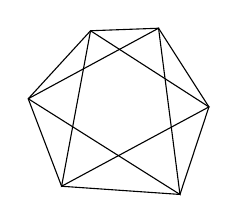
\begin{tikzpicture}[x=0.008cm,y=-0.008cm]
\draw (0,108)--(99,0)--(207,-4)--(287,121)--(241,260)--(53,247)--cycle;
\draw[thin] (0,108)--(207,-4)--(241,260)--(0,108);
\draw[thin] (99,0)--(53,247)--(287,121)--(99,0);
\end{tikzpicture}}

\[
\unsure{\nu|v}(\lambda)\nu(\lambda^{-1})\overset{?}{=}1
\]

\[
\begin{aligned}
\lambda^{-2}\nu(\lambda)&=\nu(\lambda^{-1})\overset{?}{=}\nu(\lambda)^{-1}\\
&\nu(\lambda)^2=\lambda^2\quad\overset{\text{donc}}{\Longrightarrow}\boxed{\nu(\lambda)\in(\mathbb Z/n\mathbb Z)^*}
\end{aligned}
\]

% archive sheet number: 290
